%!LW recipe=pdflatex-bibtex
\documentclass[a4paper,10pt]{article}

% ============================================================
% Common all-in-one homework / notes template (pdfLaTeX)
% The package set is intentionally broad for daily reuse.
% ============================================================
\usepackage{multicol}
\usepackage[left=1in,right=0.75in,top=0.9in,bottom=0.9in]{geometry}
\usepackage{microtype}

% Encoding and fonts
\usepackage[T1]{fontenc}
\usepackage[utf8]{inputenc}
\usepackage{newtxtext}

% Colour is loaded early because listings, TikZ, soul, and hyperref use it.
\usepackage{xcolor}

% Mathematics
\usepackage{amsmath,amssymb,amsthm}
\usepackage{mathtools}
\usepackage{newtxmath}
\usepackage{bm}
\usepackage{esint}
\usepackage{tensor}
\usepackage{stmaryrd}
\usepackage{bussproofs}

% Algorithms and code
\usepackage{algorithm}
\usepackage{algpseudocode}
\usepackage{listings}
\usepackage{fvextra}
\usepackage{mdframed}

% Markdown/Pandoc conversion support
\providecommand{\tightlist}{\setlength{\itemsep}{0pt}\setlength{\parskip}{0pt}}
\usepackage{longtable}

% Physics and engineering
\usepackage{siunitx}
\sisetup{unit-mode=text}

% Document structure and layout helpers
\usepackage{titling}
\usepackage{titlesec}
\usepackage{float}
\usepackage{enumitem}
\usepackage{setspace}
\usepackage{fancyhdr}
\usepackage{needspace}

% Tables and figures
\usepackage{graphicx}
\usepackage{caption}
\usepackage{subcaption}
\usepackage{tabularx}
\usepackage{booktabs}
\usepackage{array}
\usepackage{multirow}

% Drawing
\usepackage{tikz}
\usepackage{tikz-cd}
\usepackage{pgfplots}
\pgfplotsset{compat=1.18}

% Highlighting and boxes
\usepackage{soul}
\usepackage{tcolorbox}
\tcbuselibrary{breakable,skins}

% Numeric citation style for ordinary technical homework/reports.
% Formal IEEE/APA/ACM templates use their own bibliography systems instead.
\usepackage[numbers,sort&compress,square]{natbib}

% Hyperref is deliberately near the end.
\usepackage{hyperref}
\usepackage{bookmark}
% Color specifications transcribed from the user's uploaded palette image (2026-11-11).
\definecolor{ResearchPeach}{HTML}{FAD6C9}
\definecolor{ResearchSage}{HTML}{B0C6A8}
\definecolor{ResearchIvory}{HTML}{FAF5E8}
\definecolor{ResearchBlue}{HTML}{92B3CD}
\definecolor{ResearchRose}{HTML}{D99DA3}
\definecolor{ResearchMint}{HTML}{D0E3DB}
\definecolor{ResearchSlate}{HTML}{A6B3C0}
\definecolor{ResearchStone}{HTML}{E8E2DB}

% Readable muted link color derived from the eight-color project palette.
\colorlet{ResearchLink}{ResearchBlue!35!black}
\hypersetup{
  colorlinks=true,
  linkcolor=ResearchLink,
  citecolor=ResearchLink,
  urlcolor=ResearchLink,
  pdfborder={0 0 0}
}

% ============================================================
% Common commands
% ============================================================
\algnewcommand{\Initialize}{\State\textbf{Initialize:} }
\DeclareMathOperator*{\argmin}{arg\,min}
\DeclareMathOperator*{\argmax}{arg\,max}
\DeclareMathOperator{\rank}{rank}
\DeclareMathOperator{\tr}{tr}
\DeclareMathOperator{\spanop}{span}

% Calculus / analysis
\newcommand{\pd}[2]{\frac{\partial #1}{\partial #2}}
\newcommand{\dd}{\mathop{}\!\mathrm{d}}
\newcommand{\dx}{\,\mathrm{d}x}
\newcommand{\limit}[2]{\lim_{#1\to #2}}

% Cross-references
\newcommand{\eq}[1]{Eq.~\eqref{#1}}
\newcommand{\fig}[1]{Figure~\ref{#1}}
\newcommand{\tab}[1]{Table~\ref{#1}}

% Physics and vectors
\newcommand{\vect}[1]{\vec{#1}}
\newcommand{\Vect}[1]{\overrightarrow{#1}}
\newcommand{\grad}{\nabla}
\providecommand{\degree}{^{\circ}}

% Number systems and linear algebra
\newcommand{\R}{\mathbb{R}}
\newcommand{\C}{\mathbb{C}}
\newcommand{\N}{\mathbb{N}}
\newcommand{\bvec}[1]{\mathbf{#1}}
\newcommand{\mat}[1]{\begin{bmatrix}#1\end{bmatrix}}
\newcommand{\pmat}[1]{\begin{pmatrix}#1\end{pmatrix}}
\newcommand{\trans}{^{\mathsf T}}
\newcommand{\inv}{^{-1}}

% Probability and statistics
\newcommand{\Prob}[1]{\mathbb{P}\!\left(#1\right)}
\newcommand{\Exp}[1]{\mathbb{E}\!\left[#1\right]}
\newcommand{\Var}[1]{\operatorname{Var}\!\left(#1\right)}
\newcommand{\Cov}[1]{\operatorname{Cov}\!\left(#1\right)}
\newcommand{\indep}{\mathrel{\perp\!\!\!\perp}}
\newcommand{\Norm}{\mathcal{N}}
\newcommand{\Bin}{\operatorname{Bin}}
\newcommand{\Poi}{\operatorname{Pois}}
\newcommand{\yhat}{\hat{y}}
\newcommand{\betahat}{\hat{\beta}}

% Listings
\lstset{
  basicstyle=\small\ttfamily,
  breaklines=true,
  breakatwhitespace=false,
  backgroundcolor=\color{gray!5},
  frame=single,
  framesep=3pt,
  xleftmargin=5pt,
  xrightmargin=5pt,
  lineskip=0.5pt,
  showstringspaces=false
}

% Highlight colours
\definecolor{refblue}{HTML}{A3C4F3}
\definecolor{repgreen}{HTML}{C8E6C9}
\definecolor{transorange}{HTML}{FFD54F}
\definecolor{subviolet}{HTML}{E1BEE7}
\definecolor{ellipgray}{HTML}{E0E0E0}
\newcommand{\refhl}[1]{\sethlcolor{refblue}\hl{#1}}
\newcommand{\rephl}[1]{\sethlcolor{repgreen}\hl{#1}}
\newcommand{\transhl}[1]{\sethlcolor{transorange}\hl{#1}}
\newcommand{\subhl}[1]{\sethlcolor{subviolet}\hl{#1}}
\newcommand{\elliphl}[1]{\sethlcolor{ellipgray}\hl{#1}}

% Theorem environments
\newtheorem{theorem}{Theorem}
\newtheorem{lemma}[theorem]{Lemma}
\newtheorem{corollary}[theorem]{Corollary}
\theoremstyle{definition}
\newtheorem{definition}[theorem]{Definition}
\newtheorem{example}[theorem]{Example}
\theoremstyle{remark}
\newtheorem{remark}[theorem]{Remark}

% Homework and notes structures
\newcounter{problem}
\renewcommand{\theproblem}{\arabic{problem}}
\NewDocumentEnvironment{problem}{O{}}{%
  \par\addvspace{1.1\baselineskip}%
  \needspace{3\baselineskip}%
  \refstepcounter{problem}%
  \noindent\textbf{Problem \theproblem%
    \if\relax\detokenize{#1}\relax\else
      \enspace\textperiodcentered\enspace #1%
    \fi}\par\nobreak
  \vspace{0.25em}\hrule height 0.35pt
  \vspace{0.45em}\noindent\ignorespaces
}{%
  \par\addvspace{0.8\baselineskip}\ignorespacesafterend
}

\NewDocumentEnvironment{solution}{}{%
  \par\needspace{2\baselineskip}%
  \noindent\textbf{Solution.}\par\nobreak
  \vspace{0.2em}\noindent\ignorespaces
}{%
  \par\addvspace{0.8\baselineskip}\ignorespacesafterend
}

% Opt-in notes mode: only Definition gains the restrained blue treatment.
\newcommand{\EnableNotesMode}{%
  \tcolorboxenvironment{definition}{%
    enhanced jigsaw,
    breakable,
    colback=refblue!8!white,
    frame hidden,
    borderline west={0.8pt}{0pt}{refblue!75!black},
    boxsep=0pt,
    left=6pt,
    right=4pt,
    top=4pt,
    bottom=4pt,
    before skip=0.75\baselineskip,
    after skip=0.75\baselineskip
  }%
}

% Keep title, author, and running-header text in one place.
\newcommand{\documenttitle}{Truth Table to Circuit: A Research Trial Log}
\newcommand{\documentshorttitle}{Stage 1 Research Trial Log}
\newcommand{\documentauthor}{Jincan LI and Zeyun DU}
% The title page stays plain; this compact running header begins on page 2.
\newcommand{\runningtitle}{\documentshorttitle}
\newcommand{\runningauthor}{\documentauthor}
\setlength{\headheight}{14pt}
\fancypagestyle{mainrunning}{%
  \fancyhf{}%
  \fancyhead[L]{\footnotesize\itshape\runningtitle}%
  \fancyhead[R]{\footnotesize\runningauthor\enspace\textperiodcentered\enspace\thepage}%
  \renewcommand{\headrulewidth}{0.3pt}%
}
\pagestyle{mainrunning}

\begin{document}
\begin{titlepage}
\thispagestyle{empty}
\vspace*{1.8cm}
{\noindent\sffamily\color{ResearchBlue}\rule{\textwidth}{4pt}}\par
\vspace{1.15cm}
{\Huge\bfseries Truth Table to Circuit}\par\vspace{0.3cm}
{\LARGE A Research Trial Log\par}
\vspace{.5cm}
{\large Stage 1: from exact construction to evidence-based research decisions\par}
\vspace{1cm}
{\large UFUG2106 Discrete Mathematics Project\par}
\vspace{0.45cm}
{\large Research record through Round 6.1 --- 11 November 2026\par}
\vfill
\begin{tcolorbox}[colback=ResearchIvory,colframe=ResearchSlate,arc=2mm]
\textbf{Purpose.} This document records the \emph{path of reasoning}: what prompted each new algorithm, why the mathematical construction works, what the measurements show, and why the next experiment followed. It is intended for later self-study and transparent public research presentation. It is \emph{not} a replacement for the shorter Stage 1 technical report or for the primary evidence ZIPs.
\end{tcolorbox}
\vfill
\textbf{Version status:} Stage 1 research record v1.0, backed by the frozen Round 5.1 research source and the archived experimental record.\par
\end{titlepage}
% The round-level contents deliberately suppress the many nested subsections.
\setcounter{tocdepth}{1}
\tableofcontents
\clearpage

\section{How to read this record}
This log is intentionally more explanatory than a conventional technical paper. A reader need not know BDDs, implicants, or logic synthesis in advance. We begin with complete truth tables and the three allowed gates, then explain how each design limitation motivates the next technique. Whenever a mathematical identity is used, we distinguish that \emph{the Boolean function is preserved} from the separate empirical claim that \emph{the resulting circuit is cheaper or faster to synthesize}.

The research was not one straight sequence of uniformly better algorithms. Some changes reduced area at considerable runtime cost; a few optimization proposals were not retained. Consequently, the final architectural choice is not simply ``the version with the smallest aggregate area.'' Round 5.1 is retained as the principal efficiency candidate, while Round 4.1 Strict and Rounds 6.0/6.1 provide informative alternative points on the engineering tradeoff.

\subsection{Two reading routes}
Readers who are new to logic synthesis should begin with the synthesis problem and the recurring three-input, two-output example, then follow Rounds 1--3 to see why representation and timing analysis are needed. Readers primarily interested in the engineering decisions can begin with the research map, examine the paired runtime and cut-rewriting results in Rounds 4.1--6.1, and finish with the evidence and reflection sections. Both routes rely on the same definitions and archived measurements; the shorter Technical Report presents the selected method rather than every development turn.

\subsection{What the metrics do and do not mean}
For a legal netlist $G$ with gate-type areas $a_t$ and delays $d_t$, the output-file area is
\begin{equation}\label{eq:logarea}
 A(G)=\sum_{t\in\{\mathrm{AND2},\mathrm{OR2},\mathrm{NOT}\}}N_t(G)a_t.
\end{equation}
Every emitted gate is charged exactly once, even if its output fans out to several consumers. The network delay, in contrast, is a \emph{critical-path} quantity:
\begin{equation}\label{eq:logdelay}
 T(v)=\max_{u\in\mathrm{fanin}(v)}T(u)+d_{\operatorname{op}(v)},\quad D(G)=\max_{y\in\mathrm{outputs}}T(y),
\end{equation}
with source arrival zero (for NOT, the maximum has one argument). Finally, the synthesizer runtime $T_{\rm synth}$ is the wall-clock time of the \emph{program constructing $G$}, not the propagation delay $D(G)$. These are dimensionally and conceptually different. The official evaluator additionally distinguishes the Boolean/format/limit status \texttt{PASS} from \texttt{target\_met}. The provided project instructions and evaluator interface~\cite{coursehandout} do not reveal a numerical grading formula, so our totals across cases are engineering diagnostics rather than an official grade.

\subsection{A short notation guide}
The same symbols recur at different stages of the project. The distinction between the Boolean function and its implementation matters throughout:
\begin{table}[H]
\centering\small
\caption{Notation used throughout the trial record. These are definitions, not performance claims.}\label{tab:notation}
\begin{tabularx}{\textwidth}{@{}p{.25\textwidth}X@{}}\toprule
\textbf{Symbol} & \textbf{Meaning}\\\midrule
$F$ or $f$ & Desired Boolean output vector or a single Boolean function from the input truth table.\\
$G$ & Concrete, directed acyclic gate network realizing $F$.\\
$A(G)$ & Charged area of all live gates in $G$ (shared gates count once).\\
$D(G)$ & Maximum output arrival time; a property of the circuit.\\
$T_{\rm synth}$ & Wall-clock runtime of the synthesis \emph{program}, not the circuit delay.\\
$T(v),R(v)$ & Arrival time and required arrival time of a node in a fixed network.\\
$\rho(G)$ & The program's internal lexicographic candidate ranking, not an official score.\\
\bottomrule\end{tabularx}
\end{table}

\subsection{The frozen solver's ranking is not the evaluator's score}
The Round 5.1 code uses a lexicographic tuple
\[
\rho(G)=\big(\max(0,D-D_{\rm target}),\ \mathbf1_{D\le D_{\rm target}}A,\ D,\ A\big).
\]
A feasible candidate is ranked by area and then delay; an infeasible candidate is first ranked by how badly it misses the target. This tuple is an \emph{internal engineering heuristic}. The evaluator's public CLI exposes limits and performance metrics, but not a numerical grade formula. A clock-dependent search also means improving runtime can change which candidates finish before the cutoff; identical fixed-candidate semantics do not logically force identical final output bytes.

\subsection{The narrative contract}
Each iteration answers six questions: (1) What observable problem remained? (2) Which mathematical property suggested an answer? (3) What was implemented, rather than merely proposed? (4) What independent check supports correctness? (5) What happened to area, delay and runtime under measured conditions? (6) How did this evidence change the next decision? Formal results are statements about functions or algorithms under assumptions; benchmark claims are observations of frozen implementations.

\subsection{The research map: decisions, not just versions}
A conventional changelog would list features in implementation order. A research notebook should reveal why an observation made the next experiment reasonable. Table~\ref{tab:decisionmap} summarizes that logic; each transition will later be examined with its precise mathematical condition and supporting evidence.
\begin{table}[H]
\centering\footnotesize
\caption{A question-led map of the Stage 1 research path. ``Observation'' denotes the development evidence prompting the next question, not a controlled causal effect.}\label{tab:decisionmap}
\begin{tabularx}{\textwidth}{@{}p{.13\textwidth}X X@{}}\toprule
\textbf{Move} & \textbf{Observation to explain} & \textbf{Next hypothesis}\\\midrule
R1 $\to$ R2 & Correct netlists can still miss delay targets. & Change decision orders and mapping forms, not the truth function.\\
R2 $\to$ R3 & Better representations still leave costly shared gates and slack unused. & Optimize the costed DAG under global timing requirements.\\
R3 $\to$ R4 & A local De Morgan choice ignores shared polarity across consumers. & Evaluate phase and shallow algebra jointly with real DAG costs.\\
R4 $\to$ R4.1 & Additional candidates yield small area gains but expensive searches. & Make Area--Runtime tradeoffs explicit.\\
R4.1 $\to$ R5--5.1 & Repeated structure building and text processing waste search time. & Preserve candidate semantics while eliminating recomputation.\\
R5.1 $\to$ R6 & A fast mapping framework need not exhaust local Boolean alternatives. & Resynthesize bounded cuts under exact full-network costs.\\
R6.0 $\to$ R6.1 & Valid area gains do not justify the measured runtime. & Cache and prioritize cuts with a fixed search budget; accept or stop.\\\bottomrule
\end{tabularx}
\end{table}

\noindent\textbf{What would have counted as failure?} A proposed new mapping would be rejected if it broke functionality, missed required delay targets without a compensating purpose, or exhausted permitted resources. An engineering refactor would not qualify as an area-preserving speedup merely because it was faster on one selected case: it had to retain complete official results and survive paired and additional-function checks. These tests do not prove hidden-case performance, but they make the research decisions falsifiable.

\section{Starting point: what is the real synthesis problem?}
A complete truth table for $F:\{0,1\}^n\to\{0,1\}^m$ contains $2^n$ input assignments and $m$ output bits per row. One can always write a sum of minterms: for each row on which $f=1$, form the conjunction of the required input literals, then OR all such conjunctions. The construction is exact, but it can repeat the same combinations, use many NOT gates, and produce long chains of ANDs and ORs. This shows the central tension: \emph{existence of a legal circuit} is elementary, while finding a good shared circuit is not.

The allowed gate set is not a library of all Boolean operations. A multiplexer, XOR, or majority gate can appear in an abstract derivation but must be lowered to AND2, OR2, and NOT, each priced by the current test case. For example,
\begin{equation}
 a\oplus b=(a\lor b)\land\neg(a\land b).
\end{equation}
This identity proves implementability, but not that its right-hand side has optimal area or delay. Gate sharing and heterogeneous prices determine which realization is preferable. A gate appearing in two output expressions should ideally be computed once and reused; however, choosing what to share can affect the critical path.

The frozen Round 5.1 source reads the optional runtime limit but does not explicitly parse or enforce a separately supplied ninth-line RAM limit. The evaluator may enforce memory externally; a successful published run or one Peak RSS sample is not a universal guarantee. The full truth table alone requires reading $\Omega(m2^n)$ input bits, and ROBDD size and heuristic search costs can be exponential in the worst case.

A second early realization is that the optimum is constrained rather than scalar. The natural question is whether we can reduce $A(G)$ while keeping $D(G)\le D_{\rm target}$ and avoiding program limits. We will repeatedly return to this distinction.

\begin{tcolorbox}[colback=ResearchIvory!75,colframe=ResearchSlate,title=Four levels of objects: keep them separate]
The \emph{truth table} is the specification of $F$. A \emph{BDD} is one compact way to represent that function by recursive decisions. A \emph{gate DAG} is the actual implementation with fanout, prices, and timing. Finally, the \emph{synthesizer} is the program searching for such DAGs and consuming CPU time and memory. A theorem about one level must not silently be turned into a performance claim about another.
\end{tcolorbox}

\section{A recurring three-input, two-output example}
This running example will distinguish Boolean reasoning, structural representation and priced implementation throughout the log. Let
\[
 f_1=(a\land b)\lor(\neg a\land c),\qquad f_2=f_1\lor b.
\]
The complete table, ordered by $(a,b,c)$, is:
\begin{center}\small
\begin{tabular}{ccc|cc}\toprule
$a$&$b$&$c$&$f_1$&$f_2$\\\midrule
0&0&0&0&0\\0&0&1&1&1\\0&1&0&0&1\\0&1&1&1&1\\
1&0&0&0&0\\1&0&1&0&0\\1&1&0&1&1\\1&1&1&1&1\\\bottomrule
\end{tabular}
\end{center}
\textbf{Shannon step.} Restriction at $a=0$ gives $f_1=c$ and $f_2=b\lor c$; restriction at $a=1$ gives $f_1=f_2=b$. Therefore the two output BDDs share the $b$ cofactor. Yet a shared \emph{BDD node} is not a physical gate, and shared gate placement must be decided after mapping.

To make the reduction visible, the root decisions can be written as
\[
\begin{array}{c|cc}
 & a=0 & a=1\\\hline
f_1 & c & b\\
f_2 & b\lor c & b
\end{array}.
\]
One decision graph with root $a$ for each output therefore points to the \emph{same} residual subproblem $b$ in both high branches. The equality of two cofactors is a mathematical reason for merging them; no heuristic guess is involved. It does \emph{not} imply that a post-mapping hardware node has to be reused at every possible location.

\textbf{A legal netlist.} Using ID $0$ for constant zero and IDs $1,2,3$ for $a,b,c$, take
\[
\begin{array}{c|l}
\text{ID}&\text{gate and inputs}\\\hline
4&\mathrm{NOT}(1)\\
5&\mathrm{AND2}(1,2)\\
6&\mathrm{AND2}(4,3)\\
7&\mathrm{OR2}(5,6)\\
8&\mathrm{OR2}(7,2)
\end{array}
\qquad(y_1,y_2)=(7,8).
\]
For illustrative areas $a_{\mathrm{AND2}}=2$, $a_{\mathrm{OR2}}=3$, $a_{\mathrm{NOT}}=1$, the area is $2(2)+2(3)+1=11$. Let the respective gate delays be $2,2,1$. Forward arrival propagation gives $T(4)=1$, $T(5)=2$, $T(6)=3$, $T(7)=5$ and $T(8)=7$, hence network delay $7$. With target $8$, $R(8)=8$ and $R(7)=\min\{8,8-2\}=6$, so gate $7$ has slack $R(7)-T(7)=1$ along the path to output $8$. Although $7$ is itself the first primary output, it is also a fanin of gate $8$: its required time is therefore \emph{stricter than the nominal output target}. This provides a concrete example of why multi-output sharing matters in the backward timing recurrence.

\textbf{A useful surprise.} Absorption changes $f_2$ to $b\lor(\neg a\land c)$. Gate $8$ can therefore use inputs $(2,6)$ without changing any other line, producing the same two Boolean outputs and the same area, but output $f_2$ then arrives at time $5$. This is not a global optimum proof; it is a controlled illustration of why algebra, fanout and timing must be considered jointly.

\textbf{What happens to required time after a rewrite?} After absorbing $f_2$ into the direct gate $8=\mathrm{OR2}(2,6)$, gate $7$ no longer feeds gate $8$, although it remains the first primary output. Its \emph{new} required time becomes $R'(7)=8$ rather than $6$. Thus a valid rewrite can change the fanout graph and the required-time constraints even when it preserves both Boolean outputs. This is exactly why old required times are local proof tools for a \emph{fixed-boundary} rewrite, not numbers that may safely be reused after arbitrary restructuring.

\section{Round 1: obtain an indisputably correct construction}
\subsection{Observation and motivation}
Before comparing elaborate heuristics, we need a constructor that never relies on guessing hidden circuit structure. A complete table does not disclose the network that produced it, and many distinct networks can implement exactly the same function. The logical target should therefore be \emph{equivalence to the table}, not reconstruction of a hypothetical unique original gate diagram.

\subsection{The mathematical step: Shannon decomposition}
Pick any variable $x_i$ and restrict the function to its two possible values: $f_0=f|_{x_i=0}$ and $f_1=f|_{x_i=1}$. The Shannon identity, a foundation of switching-network synthesis~\cite{shannon1949}, is
\begin{equation}\label{eq:logshannon}
 f=\neg x_i\land f_0\;\lor\;x_i\land f_1.
\end{equation}
Why is this true? If $x_i=0$, the first conjunction reduces to $f_0$ and the second to zero; if $x_i=1$, the roles exchange. These two cases exhaust the domain. Repeatedly applying (\ref{eq:logshannon}) reduces every function to constants at the leaves and is therefore a constructive correctness argument.

But a full Shannon \emph{tree} may represent the same cofactor in many branches. Consider a function whose truth values no longer depend on a variable after earlier decisions; continuing to branch on that variable is redundant. Another possibility is that two different branches lead to the identical remaining function. These are representation-level redundancies, not exotic Boolean identities.

\subsection{Reduced Ordered Binary Decision Diagrams}
Fix a variable order $\pi$. A BDD node stores its decision variable and the references to its low and high cofactors. We apply two exact reductions: (i) if the two child references are equal, skip that decision; (ii) if an identical node with the same variable and child references exists, reuse it from a unique table. The result is a shared DAG, not merely a binary tree. Bryant's ROBDD framework explains why fixed ordering and reduction give a canonical function representation~\cite{bryant1986}.

\begin{theorem}[Structural correctness of reduced Shannon DAGs]
If every terminal has the correct constant value and every decision node computes (\ref{eq:logshannon}), merging nodes of equal triples and deleting nodes with equal children leaves every output function unchanged.
\end{theorem}
\begin{proof}
The full decision expansion computes the table by repeated case analysis. Merging two identical triples merges identical decision expressions. When the low and high child coincide, $\neg x f_0\lor xf_0=f_0$, so the parent is redundant. Apply these identities at each reduction step.\end{proof}

\subsection{Implementation and evidence}
The baseline lowers decisions to the allowed physical gates, shares equal gate expressions via structural hashing, and outputs topologically ordered IDs. The Round 1 WSL evidence is 25/25 official PASS but only 12/25 cases meeting the target delay; summed area is 1,103,455. The independent checker additionally verified the outputs under its own exhaustive-or-sampled procedure.

\begin{tcolorbox}[colback=ResearchPeach!35,colframe=ResearchRose,title=Decision after Round 1]
\textbf{Learning:} the algorithm is correct, but correctness alone says nothing about whether its variable order, sharing pattern and gate depth are good. Next, keep the exact Shannon foundation but widen the space of equivalent realizations.
\end{tcolorbox}

\section{Round 2: representation is an optimization variable}
\subsection{Why a smaller BDD need not imply a smaller circuit}
A BDD is an abstract decision representation; the assignment asks for a priced AND/OR/NOT netlist. Two BDDs encoding the same function can have very different numbers of decision nodes, but even fewer decision nodes need not imply cheaper \emph{mapped} gates. One structure may expose common AND subexpressions, another may induce many NOT gates, and a third may admit more balanced evaluation. Thus variable ordering and mapping must be evaluated \emph{after} lowering into the actual library.

\subsection{Influence-based variable ordering}
A natural way to choose a decision variable is to ask whether changing it frequently changes the output. For a single Boolean function,
\begin{equation}
 I_i(f)=\frac{1}{2^{n-1}}\sum_{x_{-i}}\mathbf1\{f(x_{-i},0)\ne f(x_{-i},1)\}.
\end{equation}
A variable with large influence is frequently decisive. The heuristic places such variables earlier in one candidate order. This is a plausible structural guide, \emph{not} an optimality theorem: sensitivity and BDD node count are different notions, and neither captures weighted gate area by itself.

\paragraph{Compute influence instead of taking it on faith.} In the running example, $f_1$ chooses $c$ when $a=0$ and $b$ when $a=1$. Flipping $a$ changes the output precisely when $b\ne c$, which occurs on two of the four $(b,c)$ assignments. Therefore $I_a(f_1)=1/2$. Flipping $b$ changes $f_1$ when $a=1$, while flipping $c$ changes it when $a=0$; so $I_b(f_1)=I_c(f_1)=1/2$ as well. Influence cannot distinguish the selector from either data signal for this function. By contrast, $f_2=b\lor(\neg a\land c)$ has $I_b(f_2)=3/4$ and $I_a(f_2)=I_c(f_2)=1/4$. The combined influence ordering can be useful but is inevitably sensitive to how multiple outputs are aggregated. It does not know the actual gate prices or the quality of downstream sharing.

\subsection{Two-level Shannon expansion}
One first-level decision may create a long chain of nested multiplexor-like logic. The next idea is to expand two levels at once, possibly choosing different second variables in the two branches. Formally,
\begin{align*}
 f={}&\neg x\land(\neg u\land f_{00}\lor u\land f_{01})\\
 &\lor x\land(\neg v\land f_{10}\lor v\land f_{11}).
\end{align*}
The derivation simply substitutes Shannon's identity into both cofactors. Its advantage is structural: four gated terms can often be computed in parallel and combined with a balanced OR structure, which may shorten the critical path. Its disadvantage is equally important: an expansion can duplicate shared subfunctions and inflate area. It belongs in a \emph{portfolio}, not as an unconditional rewrite.

\subsection{Small-support SOP and POS}
The next route does not begin with a BDD at all. A variable is \emph{essential} if its two cofactors differ. When a function depends only on a few essential variables, directly enumerate cubes (partial assignments), derive prime implicants, and select a greedy cover of the function's on-set. An SOP is exact if every selected cube implies the function and their union covers all true minterms. This is worth proving as two inclusions. Every selected cube lies inside the on-set, hence the SOP never outputs $1$ where $f=0$; coverage ensures the SOP never outputs $0$ where $f=1$. Consequently it agrees with $f$ on the entire domain. A POS-like implementation can be obtained by covering the complement and negating its result. The optimization is incomplete because greedy cover is not guaranteed minimal, and prime enumeration can become exponential, so the implementation restricts support size. These are familiar issues in classical two-level logic minimization~\cite{brayton1984}.

\paragraph{A cover on the running example.} Since $f_2=b\lor(\neg a\land c)$, the cube $b$ covers all rows with $b=1$, while $\neg a\land c$ covers the remaining true row with $a=0,b=0,c=1$. Both cubes imply $f_2$, and together they cover its complete on-set: the expression is therefore exact, not merely a plausible simplification. Distributivity also yields the POS
\[
 f_2=(b\lor\neg a)\land(b\lor c).
\]
Neither canonical form is guaranteed to be cheapest after mapping: an AND2, OR2, or NOT may have different prices, and some of their subexpressions may already exist in another output's graph.

\begin{example}[Factoring is a mapping choice]
The SOP $(a\land b)\lor(a\land c)$ is logically equal to $a\land(b\lor c)$. The first exposes two independent AND terms; the second shares $a$ and may use fewer gates. Which has lower delay depends on $d_{\land}$, $d_{\lor}$ and the incoming arrivals. Thus algebraic equality is a correctness fact, while its desirability is a cost fact.
\end{example}

\subsection{Portfolio selection and outcome}
Round 2 compares a fixed collection of candidates built from alternative decision orders, two-level expansion and small-support implicant forms, then measures their exact final netlist costs. The WSL result has 25/25 PASS and 25/25 target delays, with summed area 790,243, a reduction of roughly 28.4\% from Round 1. The search itself costs more runtime: median WSL runtime increases from 5.455 ms to 36.427 ms across those separately archived runs. Since these are not an interleaved pairing, the numbers indicate scale, not an exact causal speed ratio.

\begin{tcolorbox}[colback=ResearchSage!25,colframe=ResearchSage,title=Decision after Round 2]
\textbf{Learning:} representation diversification succeeds at closing the timing-feasibility gap. But much area remains, and an alternative can become more useful when its negated form or downstream slack is exploited. Next, look at the entire shared graph under case-specific prices and deadlines.
\end{tcolorbox}

\section{Round 3: account for complements, shared algebra and timing slack}
\subsection{Complemented edges: negation is information before it is a gate}
If $g=\neg f$, it seems wasteful to store two unrelated Boolean subgraphs representing $f$ and $g$. A complemented-edge BDD reference stores a regular node identity plus one inversion bit. The graph can share the same structural nodes, while the inversion bit carries the semantic complement. To prevent multiple redundant encodings, the unique table normalizes one child-complement convention before interning nodes. This is a representation optimization; when mapped into physical AND2/OR2/NOT, a required inverter must still be emitted or shared and charged.

An affine detector also recognizes functions $c\oplus\bigoplus_{i\in S}x_i$. If the high cofactor equals the negation of the low cofactor, Shannon decomposition reduces to XOR with the decision variable. To check the algebra, write $q=f|_{x=0}$ and $f|_{x=1}=\neg q$; then
\[
 f=(\neg x\land q)\lor(x\land\neg q)=x\oplus q.
\]
This recognizes one XOR-shaped decision, not automatically an arbitrary global affine function; full affine recognition requires the appropriate recursive consistency across the remaining variables. It can allow structured balanced XOR constructions, all lowered through legal gates. It can help parity-like truth tables that ordinary BDD mapping handles awkwardly.

\subsection{Why timing slack changes the optimization problem}
Imagine a network whose target delay is 30 but whose actual delay to an output is 22. A gate-level rewrite that increases an intermediate arrival by 2 is not automatically harmful if every downstream path still finishes by 30. A greedy ``never increase any arrival'' policy leaves potentially cheaper gates unexplored.

The more principled tool is \emph{required time}. Assign $R(y)=D_{\rm target}$ at each primary output and propagate deadlines backward:
\begin{equation}\label{eq:logrequired}
 R(u)\gets\min\{R(u),R(v)-d(v)\}
 \quad(u\in\mathrm{fanin}(v)).
\end{equation}
A shared node receives the strictest requirement over its consumers. Its slack is $S(u)=R(u)-T(u)$. We can then consider a cheaper De Morgan mapping even if it slightly increases local delay, provided the new arrival does not exceed $R(u)$. For instance,
\begin{equation}
 a\lor b=\neg(\neg a\land\neg b)
\end{equation}
may substitute a cheap AND and shared inversions for an expensive OR. An isolated sufficient area comparison involves $a_{\lor}$ versus $a_{\land}+3a_{\neg}$, but the actual DAG cost depends on which inversions are already present and which gates stay alive due to fanout. Global remeasurement is essential.

\begin{lemma}[Fixed-boundary timing invariant]
Start from a feasible DAG $G$ and compute the old required times $R_G$ backward. Replace an internal cone by an equivalent acyclic cone with the same external boundary. If every replacement root exposed to the unchanged graph has newly computed arrival at most its old required time, and the unchanged gates preserve their old types, delays and dependency edges, the new output delay is at most the target.
\end{lemma}
\begin{proof}
Contract each new cone into its exposed root. Each such root meets the old required bound by assumption. For an unchanged gate $v$, each incoming unchanged dependency $u\to v$ obeys $R_G(u)\le R_G(v)-d(v)$. Thus by topological induction $T'(v)\le\max_u R_G(u)+d(v)\le R_G(v)$, including unary NOT with one predecessor. Every output requirement remains at most the original delay target; an output reused internally may have a strictly smaller required time.
\end{proof}
\textbf{Why the assumptions matter.} A rewrite that changes fanout, creates a new cross-cone dependency or reuses stale required times after another transformation is outside this lemma. The implementation remeasures the whole candidate DAG, and the accepted-candidate ranking provides a second engineering safeguard. A sufficient condition is not a proof of optimal area or of correctness of arbitrary rewrite code.

\subsection{Balancing, bounded search and outcome}
Associative AND/OR chains are re-parenthesized when doing so does not break essential sharing, and additional variable orders are attempted under a computation budget. Every candidate is pruned and evaluated as a complete live DAG. The archived Round 3 WSL Area is 533,705 with 25/25 PASS and 25/25 target delay; this is approximately 32.5\% below Round 2. The magnitude is a central Stage 1 result, but it is the combined effect of several features. It should not be attributed solely to required-time recovery without the corresponding ablation data.


\subsection{What the archived Round 3 ablation actually establishes}
We later recovered a development summary that was missing from the first writing draft. Rather than treating the final result as one opaque improvement, it lists concrete snapshots along an algorithmic path. Starting at the $790{,}243$-area portfolio, the successive archived snapshots record $777{,}324$ after complemented-BDD development, $770{,}195$ after affine detection, $762{,}164$ after balancing, $586{,}218$ after slack-aware recovery, $543{,}209$ after an additional reverse-order candidate, and $533{,}705$ after legacy fallback selection. All listed entries have 25 successful target checks in their respective evaluations.

\begin{figure}[H]\centering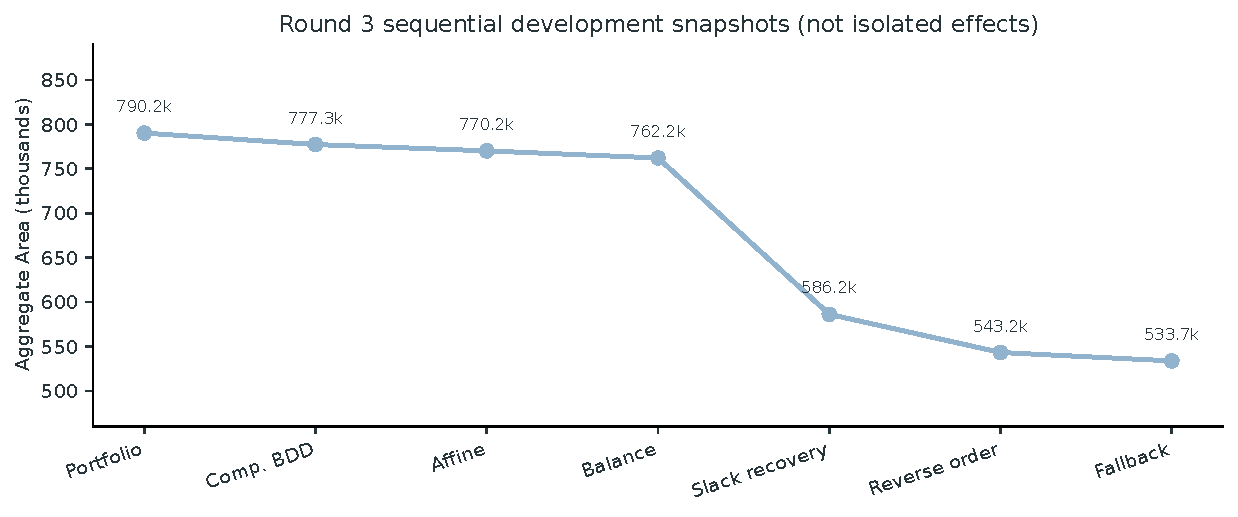
\includegraphics[width=.97\textwidth]{../shared/figures/round3_ablation_path.pdf}
\caption{The chronological Round 3 \emph{development path}; the separate implication experiment in the source CSV is deliberately not connected as though it were the next sequential stage.}\end{figure}

\textbf{Why does the distinction matter?} The $175{,}946$ difference between the balanced snapshot and the slack-recovery snapshot is an observation after a sequence of earlier changes. It illustrates why required-time reasoning was so promising, but it does not prove that activating the recovery routine on every possible prior configuration saves exactly that amount. A controlled factorial study would require frozen alternatives differing in only one feature, compiled and evaluated under matched conditions. Our source supports a strong \emph{development narrative}, not that stronger causal claim.

\begin{tcolorbox}[colback=ResearchBlue!20,colframe=ResearchBlue,title=Decision after Round 3]
\textbf{Learning:} exact Boolean identities can be used more effectively when the optimization considers shared nodes and global deadline slack. Remaining gate-level opportunities may require selecting positive or negative representations across \emph{several} fanouts. Next, explore polarity and algebraic restructuring.
\end{tcolorbox}

\section{Round 4: phase selection and algebraic rewriting}
\subsection{The missing global choice}
A physical inverter can be shared among several consumers. Therefore asking ``Should this OR gate be replaced by De Morgan?'' independently at each gate misses a global decision: which \emph{phase} of each shared signal should be stored? Define for node $v$ the phase bit $p_v\in\{0,1\}$ and stored function
\begin{equation}
 g_v=\neg^{p_v}f_v.
\end{equation}
Changing $p_v$ switches whether its children must be complemented and whether a logical AND is physically realized as an AND or, under De Morgan, as an OR on the opposite phases. For example, if a shared signal $z=u\lor v$ is stored negatively as $\neg z=\neg u\land\neg v$, an AND2 may replace an OR2 but only if the required child polarities can be produced at acceptable cost. No NOT gate is ``free'' merely because the internal BDD reference has an inversion bit. A shared NOT is paid once per realized source polarity, not once per fanout. We evaluate a surrogate phase objective and use coordinate descent as a heuristic; exact output DAG area and delay still decide whether a candidate wins. This is not a global minimum-area solver.

A second pass applies absorption and factoring across shallow gate patterns. Its gains can be small because the original Boolean structure has already been aggressively simplified. It must also avoid an incorrect inference: if one rewrites a local cone to use fewer gates, the entire netlist may remain the same size when its allegedly removed ancestors are still referenced elsewhere.

\subsection{Observed result and the search-cost warning}
Round 4 reaches summed Stage 1 area 528,910, down from Round 3 by 4,795 (approximately 0.90\%), with all 25 targets still met. But the archived WSL median synthesis time is 127.568 ms, compared with 68.486 ms for Round 3. The comparison is historical rather than same-run paired, yet the cost increase is sufficiently concerning to motivate a dedicated runtime investigation. A separate exploratory variable-order search occasionally expanded the BDD dramatically; candidate limits and fallback are needed to prevent unbounded resource consumption.


\subsection{Recovering the missing postprocessor experiment}
The newly located \texttt{postprocess\_comparison.csv} helps answer the question: was it the De Morgan phase pass or algebraic rewriting that mattered more? Applied separately to the archived Round 3 circuits, algebra only reduces total area from $533{,}705$ to $532{,}416$, while phase only reaches $533{,}378$. The two orders of composition are slightly different: phase followed by algebra gives $532{,}078$, and algebra followed by phase gives $532{,}080$. Taking the best strategy for each of the 25 cases produces $532{,}070$.

\begin{figure}[H]\centering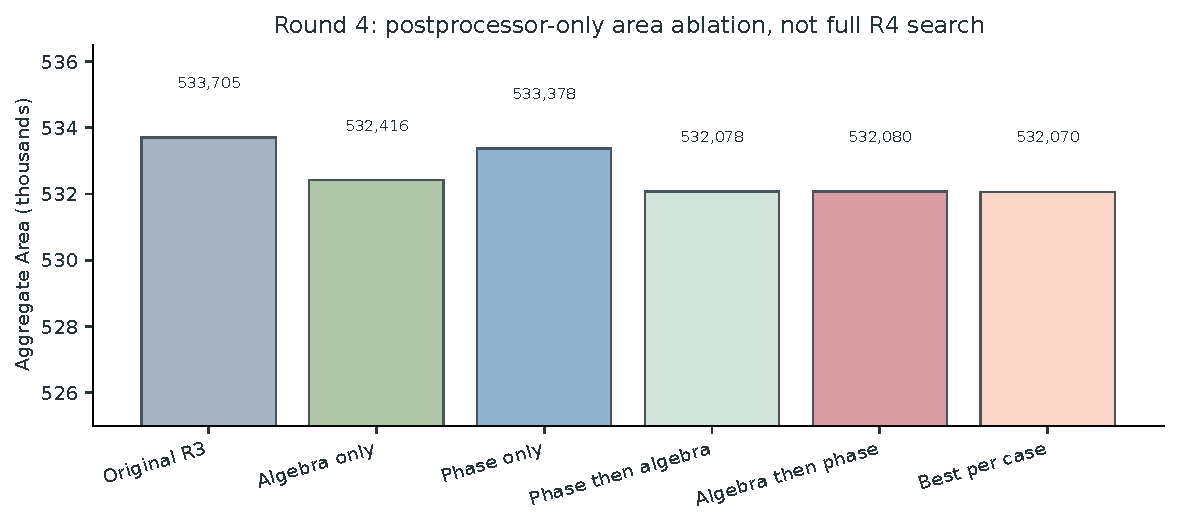
\includegraphics[width=.91\textwidth]{../shared/figures/round4_postprocess_ablation.pdf}
\caption{Round 4 postprocessing ablation. These treatments reuse the same original circuits; extra variable-order search is intentionally not included.}\end{figure}

The important insight is not that one rewriting order always wins. Both the circuit's shared fanout and the local AND/OR/NOT prices determine which candidate is best. The $532{,}070$ total uses a \emph{per-case selection}, which makes sense for a multi-candidate synthesizer but should not be confused with a single rewrite rule. The fully fledged Round 4 result of $528{,}910$ also contains further variable-order exploration. Thus the difference between $532{,}070$ and $528{,}910$ cannot be counted as a benefit of algebra and phase postprocessing alone.

\begin{tcolorbox}[colback=ResearchRose!20,colframe=ResearchRose,title=Decision after Round 4]
\textbf{Learning:} increasing the candidate pool is not free. A roughly one-percent Area gain can be purchased with disproportionately more computation. Instead of making the Boolean search even more exhaustive, first ask what work the program repeats unnecessarily.
\end{tcolorbox}

\section{Round 4.1: construct the first explicit Area--Runtime Pareto comparison}
\textbf{Counterfactual considered.} We could continue adding variable orders or polarity restarts and keep every tiny public-case area improvement. But this would spend more of a finite synthesis budget on strategies whose extra benefit had become small. The alternative was not to abandon the improved R4 circuit: it was to ask how much area a faster search would actually sacrifice.

The next experiment varies the amount of polarity postprocessing and variable-order exploration. It retains three executable configurations rather than presenting one parameter setting as universally best: \textbf{Strict} minimizes perturbation of the R4 circuit, \textbf{Balanced} accepts a tiny area change for runtime reduction, and \textbf{Fast} reduces the search further. These are meaningful \emph{Pareto alternatives}: lower runtime can require worse area, and a global criterion is impossible without knowing the actual scoring function.

Two WSL measurements report that the Balanced configuration produces Area 529,014 in both runs; its median runtime is 96.048 and 102.615 ms. Strict preserves Area 528,910, while Fast reaches Area 530,822. In the case-level data, Fast has a conspicuous area regression in \texttt{case\_018}; the small relative area-sum penalty conceals a large localized change. This demonstrates why we record per-case data and not only aggregate sums.

\paragraph{What makes two settings genuinely incomparable?} Say configuration $X$ dominates $Y$ if $A_X\le A_Y$ and $T_X\le T_Y$, with at least one strict inequality, under matched evaluations. If $X$ is smaller but slower, neither dominates the other: there is no single unambiguous winner without a scoring utility or an explicit time constraint. Strict and Balanced illustrate exactly this tension. This is a \emph{Pareto} argument, not a claim that area and milliseconds can be added together in a physically meaningful unit.

\textbf{Research decision:} Balanced becomes the candidate for engineering optimization, not because its gate area is absolutely smallest, but because its area sacrifice relative to Strict is 104 out of roughly 529,000 while lowering median runtime. We retain Strict as the area-oriented comparator.

\section{Round 5: remove recomputation before reducing search quality}
\textbf{The change of object.} Until now, the algorithm had treated the circuit as the thing being optimized. Here the \emph{synthesis program} becomes the object of analysis. This is not a semantic change to a Boolean function: we are asking whether repeated work inside the compiler can be removed before sacrificing any useful gate mapping candidate.
\subsection{A useful conceptual split}
There are two ways to accelerate a synthesis engine: \emph{delete candidate searches}, or \emph{implement the same searches more efficiently}. The latter is preferable when we already trust the candidate quality. Profiling revealed three repeated operations: multiple mapping policies rebuild the same ordered BDD; several small-support candidates recompute identical implicant covers; and every candidate's textual netlist is reparsed for area and timing estimates.

Fix the truth table $F$ and variable order $\pi$. Let $B(F,\pi)$ be its immutable BDD. If policies $\theta_1,\ldots,\theta_k$ share $\pi$, then they can all use the same BDD:
\begin{equation}
 C_i=\operatorname{Map}(B(F,\pi),\theta_i).
\end{equation}
The semantic reason is simple: BDD building depends on $(F,\pi)$, not on how a later gate mapper chooses to realize its nodes. The cache key is logically meaningful: it must distinguish different truth functions and different variable orders, and the cached graph must not be modified by downstream candidates. If the mapper mutates the shared structure, reuse becomes a correctness risk rather than a safe speedup. Likewise, cache hits justify avoiding computation, not inventing a better Boolean function. Throughout this log we use $\land$, $\lor$ and $\neg$ for Boolean connectives; $\mathrm{AND2}$, $\mathrm{OR2}$ and $\mathrm{NOT}$ denote gate types in mathematical expressions; and the corresponding monospaced tokens are reserved for literal netlist syntax. In a simplified cost model the repeated build term decreases from $kT_B$ to $T_B$. Crucially, this does \emph{not} imply a $k$-fold overall speedup when mapping or postprocessing dominates. Cached implicant covers follow the same logic: symbolic cube selections depend on the function and deterministic tie-breaking, while physical gate emission remains candidate-specific.

Round 5 also removes one provably duplicate candidate when $n>13$. In the frozen configuration the pair differed only by an implicant mode that is disabled for those dimensions, so the two candidate computations were identical. A lightweight line scanner further reduces repeated netlist-statistic overhead.

\subsection{What the paired evidence shows}
In the dedicated Round 5 WSL pairing, Round 4.1 Balanced had median synthesis runtime 87.041 ms and Round 5 had 68.861 ms, both with Area 529,014 and 25/25 correct and target-met cases. All 25 emitted netlist files in that local comparison were byte-identical. These observations support a genuine implementation-efficiency gain. However, time-based candidate cutoffs mean the same byte identity is not guaranteed under every possible timing environment; one independent container rerun had a different yet valid candidate near a deadline.

\begin{tcolorbox}[colback=ResearchMint!40,colframe=ResearchSage,title=Decision after Round 5]
\textbf{Learning:} caches remove repeated \emph{Boolean analysis}, but the engine still converts graphs to text and back as it rebalances and recovers area. If gate structure is already available, why throw it away between stages? This directly motivates typed in-memory DAGs.
\end{tcolorbox}

\section{Round 5.1: treat the netlist as a data structure, not repeated text}
\textbf{Why another implementation round?} Caching helped with BDDs and covers, but the candidates still passed through several text-to-graph and graph-to-text transformations. Those conversions have no Boolean significance; they exist only because of an inconvenient intermediate representation. Round 5.1 therefore tests whether a typed internal graph can retain the same transformation logic while making it cheaper to execute.
\subsection{The engineering hypothesis}
A text format is a good external interface but a poor internal representation for repeated graph operations. Instead of parsing a netlist for rebalancing, serializing it, then parsing again for area recovery, Round 5.1 stores a typed gate table $v\mapsto(\mathrm{op},a,b)$ and an explicit output list. Structural hashing interns identical immutable gates; reachability pruning discards dead nodes at the final serialization step. For commutative AND2/OR2 nodes the builder sorts input IDs before hash lookup. For rebalancing, a same-operation internal cone is flattened only when the interior nodes have a single consumer, while output references are included in the fanout count. An interior gate used by two consumers cannot simply be dissolved into one of them: the other consumer still needs that signal. In graph terms, only \emph{unshared} associative interiors can be freely re-parenthesized without requiring a separate replacement for the other use. This matters in a multi-output network: reusing an output as someone else's intermediate result must not cause that shared computation to be silently removed. A topological induction over gate IDs proves the functional equivalence of these associative, commutative and idempotent rewrites; a reverse reachability pass from \emph{all} output roots preserves every live shared gate.

If a new gate is created only after its fanins exist, its arrival can be stored immediately:
\begin{equation}
 T(v)=\begin{cases}
 T(a)+d_{\neg},&\operatorname{op}(v)=\mathrm{NOT},\\
 \max\{T(a),T(b)\}+d_{\operatorname{op}(v)},&\text{otherwise}.
 \end{cases}
\end{equation}
Topological induction proves this stored arrival correct. This is a real \emph{incremental arrival-time} computation, but the implementation does \textbf{not} claim incremental global area accounting. A replacement may free an entire private cone, but a gate that still serves another output remains live. Exact area is recomputed after reachability pruning to avoid charging errors.

\paragraph{Follow one gate through the builder.} The input Netlist assigns every gate an ID greater than its fanin IDs. The in-memory parser stores that ordered graph as nodes $(\mathrm{op},a,b)$; the builder can therefore compute $T(v)$ immediately after a new node is created. When two AND2 nodes receive the same two operands in opposite orders, sorting their IDs makes their hash keys identical, which is legal because $u\land v=v\land u$. The key does \emph{not} unify arbitrary Boolean-equivalent but structurally different expressions: that would require more algebraic reasoning. After transformations, the serializer traces backward from \emph{every} output, discards nodes outside the union of their ancestor sets, and renumbers the rest. Induction over this topological order explains both semantic preservation and why a gate feeding multiple outputs must be counted only once.\par
\textbf{Limits of the proof.} This reasoning assumes each local rewrite implements the intended Boolean identity and that its new dependencies remain acyclic. The actual program still needs parser validation, full-DAG rescoring and independent netlist checks; a correct identity on paper cannot rule out an indexing bug in C++.

\subsection{Why this is not just another heuristic}
Round 5.1 keeps the same mapping policies and internal cost ranking as Round 5. The typed DAG covers the high-frequency candidate balancing/recovery passes, but the final phase/algebraic alternatives still serialize and reparse netlists; the system is not entirely text-free. The aim is to change the \emph{cost of executing} the optimization, not its mathematical candidate space. Accordingly, functional identity and equal output netlists are strong regression checks. In a first WSL paired run all 25 Round 5 and 5.1 outputs were byte-identical; the second had the same per-case areas and delays. Under a clock-bounded search, this remains an empirical property rather than a cross-platform guarantee. In particular, the source uses elapsed-time checks before later modern and legacy candidates, additional postprocessor eligibility thresholds, and periodic time checks for selected BDD orders; none constitutes a hard preemption mechanism for all stages. Since the candidate set is timing-dependent, two correct executions can output different valid netlists while using the same lexicographic ranking. The comparison to Round 5.1 therefore supports an engineering-efficiency claim, not a deterministic-output or optimality theorem.

\subsection{Measured speed and generalization}
The WSL paired medians change from 72.188 to 55.488 ms in one run and 60.827 to 55.077 ms in the other. Both versions have 25/25 PASS, 25/25 target delays and total Area 529,014. The average of the two per-run medians improves from 66.508 to 55.283 ms, about 16.9\% (a descriptive two-run estimate). A mixed holdout of 80 functions and a 16-case larger set also pass the evaluator and independent checker, but the gains are distribution-dependent: small cases may see little benefit or small overhead, while larger graphs profit more from avoided parsing.

\begin{figure}[H]\centering
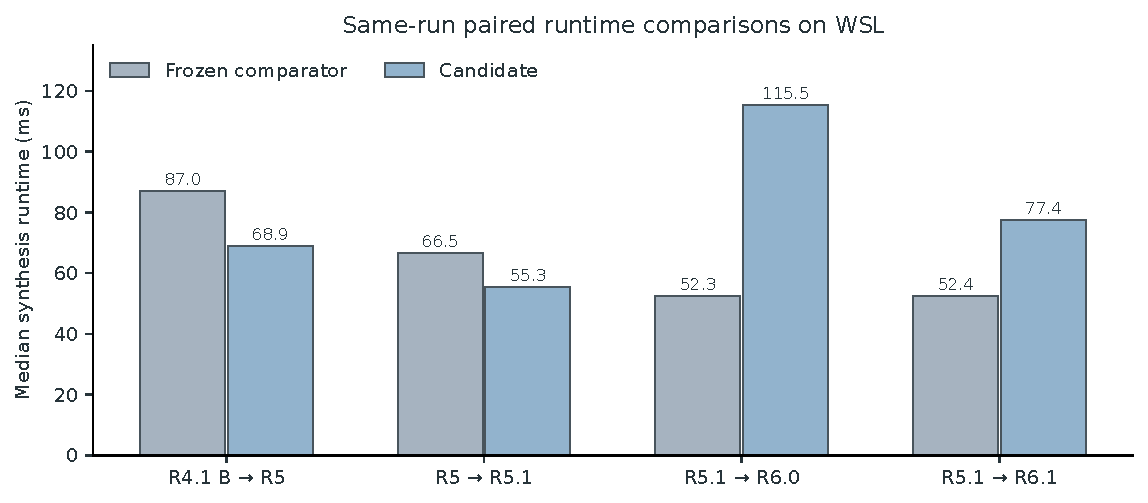
\includegraphics[width=.96\textwidth]{../shared/figures/paired_runtime.pdf}
\caption{Paired WSL comparisons from distinct recorded experiments. The figure is constructed from authentic CSV records with the bundled plotting script; inter-group medians are not interchangeable experiments.}\end{figure}

\begin{tcolorbox}[colback=ResearchBlue!18,colframe=ResearchBlue,title=Decision after Round 5.1]
\textbf{Learning:} the engineering refactor achieves another measurable runtime gain without sacrificing measured gate quality. The next research question should not be ``how many more milliseconds can be shaved?'' but ``is the chosen function decomposition leaving significant circuit-area opportunities on the table?'' Freeze this implementation as the efficiency baseline.
\end{tcolorbox}


\subsection{A limited memory snapshot: what Peak RSS says}
After the source freeze was checked on the student's own WSL installation, we ran the exact research source on the large \texttt{case\_024} as a standalone process under GNU \texttt{/usr/bin/time -v}. The terminal reported normal exit, wall-clock time $1.66$ s and peak resident memory $69{,}480$ KiB ($67.85$ MiB); the synthesizer itself reported area $124{,}475$ and delay $70$. The raw \texttt{/tmp} time log was not uploaded, so this writing archive labels the record as a student-supplied terminal transcription.

The measurement answers a narrow question: \emph{how much memory did one particular process run make resident at its peak?} It does not bound worst-case memory across the 25 official cases, does not measure all virtual-memory allocations, and must not replace the official evaluator's per-case synthesis runtime. Preserving these distinctions is part of experimental reproducibility, not a cosmetic disclaimer.

\section{Round 6.0: a change of representation, not merely another BDD order}
\textbf{Why resume Boolean optimization after engineering speedups?} A faster synthesis engine is valuable only if it gives room to seek better realizations, or if synthesis time itself is a scoring concern. The next experiment deliberately returns to gate quality: a mapped DAG can still contain locally expensive expressions that are not exposed by changing the original BDD order. This is a new hypothesis, not an extension of the caching theorem.
\subsection{Motivation: escaped local equivalences}
A BDD-derived circuit may already be compact as a BDD yet still contain local multi-gate patterns that another circuit can implement more cheaply. The new idea is to inspect \emph{the final gate DAG itself}, choose a small boundary of signals, recover the exact Boolean subfunction between that boundary and an internal output, and resynthesize the subfunction independently of the original local shape.

\subsection{What exactly is a feasible cut?}
For a chosen node $v$, a cut $C_v$ is a collection of upstream boundary nodes meeting every path backward from $v$ to a primary input. A $k$-feasible cut has at most $k$ leaves. Round 6.0 fixes $k\le4$. Treat the cut-leaf values as \emph{formal} independent variables solely when enumerating assignments. This is not probabilistic independence: the real leaf signals can be correlated, but any replacement equal on all $2^k$ formal assignments is certainly equal on the subset the surrounding circuit can actually produce.

With $k\le4$, the local truth table uses at most $2^4=16$ bits:
\begin{equation}
 M_{v,C}=\sum_{s=0}^{2^k-1}f_{v,C}(s)\,2^s.
\end{equation}
This small mask is the bridge between an arbitrary gate cone and generic Boolean synthesis; classical DAG-aware AIG rewriting offers a related but more comprehensive rewrite-library approach~\cite{mishchenko2006,abc}. Candidate realizations include SOP, complemented SOP/POS, shallow factoring and one-variable Shannon decompositions. All use AND2, OR2 and NOT. The search is \emph{not} complete and should not be called an exact minimum-area optimizer.

\subsection{Why gate sharing makes local estimates dangerous}
\paragraph{A cut mask that can be checked by hand.} Return to the example's second output $f_2=b\lor(\neg a\land c)$. Treat $(a,b,c)$ as formal cut leaves and number assignments by $s=4a+2b+c$. The rows where $f_2=1$ are $s=1,2,3,6,7$, so its 8-bit truth-function mask is
\[
 M_{f_2,\{a,b,c\}}=2^1+2^2+2^3+2^6+2^7=206=\texttt{0xCE}.
\]
A local resynthesizer can check candidate expressions against these eight bits \emph{before} considering gate costs. Equality on all formal boundary assignments guarantees equality for the actual boundary signals, even if they are not independently realizable; the guarantee is sufficient, not necessarily a minimal test. It says nothing yet about cycles, the output interface, or area.

\paragraph{Count the surviving DAG, not the rewritten text.} Let $L(G)$ be the set of gates reachable from \emph{any} primary output. With prices $a(v)$, the exact area is $A(G)=\sum_{v\in L(G)}a(v)$. If a candidate ``eliminates'' a gate which still feeds another output, that gate remains in $L(G)$ and its area is not saved. Our running example shows this sharply: after replacing gate $8$, gate $7$ is no longer used by $8$, but must remain because it is still the first output. The original and rewritten circuits both cost $11$; the benefit is delay, not area. A valid local rewrite therefore needs both semantic equality and a complete live-DAG cost check.

Suppose a cut replacement seems to save a gate $g$. If another output still references $g$, deleting one use does not eliminate its physical cost. Conversely, a rewrite can free several upstream private nodes at once. The implementation conservatively estimates removable gates through reference counts and counts the candidate local cone cost without treating speculative gates from rejected alternatives as free. Only after an actual candidate is produced does it prune and measure the complete graph, retaining it when true area drops and the deadline remains met.

\subsection{Outcome: a successful hypothesis but costly implementation}
In the user's two WSL paired runs, Round 6.0 area changes from 529,014 to 528,738 and 528,744, with 25/25 PASS and target delays. Median runtime, however, increases from 53.286 to 114.610 ms and from 51.403 to 116.351 ms. In another set of 40 generated functions, area falls from 9,709 to 9,496; in an older 80-case set it falls from 22,821 to 22,579; for 16 larger cases it falls from 157,944 to 157,440. These tests support that additional optimization opportunities exist beyond particular public case IDs, but the synthetic distributions do not prove hidden-case success.

\begin{tcolorbox}[colback=ResearchPeach!30,colframe=ResearchRose,title=Decision after Round 6.0]
\textbf{Learning:} new area savings are real, but the cost of repeatedly enumerating cuts and rebuilding equivalent cover candidates is too high. The next question should be ``can the same local search be made cheaper?'', not ``can we enlarge $k$?''
\end{tcolorbox}

\section{Round 6.1: a deliberate Go/No-Go experiment}
\subsection{Predeclared engineering constraint}
We froze $k\le4$ and made the optimization budget explicit. The cut postprocessor receives 25 ms wall-clock budget, with a second constraint linked to the per-case runtime allowance, and keeps caps on retained cuts and visited roots. The baseline Round 5.1 candidate remains available as fallback. This is \emph{not} a 25 ms bound on the whole synthesis process.

\subsection{Reuse local Boolean work}
For a four-leaf cut, a truth mask contains at most 16 bits, but the same function may appear at many locations. We cache symbolic implicant covers under
\begin{equation}
 K=(k,M,p),
\end{equation}
where $k$ is the number of formal leaves, $M$ the truth mask, and $p$ the deterministic greedy cover policy. The cache stores no actual DAG gate IDs, no fanout, and no timing data. Thus a hit preserves the symbolic Boolean cover while each candidate is re-emitted against its own physical cut leaves. Canonicalizing arbitrary input permutations would require tracking the permutation; this implementation does not silently identify them.

Cuts are also prioritized using a conservative estimate of removable \emph{private} old gates. Finally, the complete netlist is remeasured before an accepted rewrite can replace the incumbent. The method is designed to reduce wasted search, not to expand the mathematical search space.

\subsection{What the local evaluation actually concluded}
Two WSL comparisons reported Round 6.1 areas 528,854 and 528,839 versus 529,014, with full official PASS and target delay. Median synthesis runtime increased from 54.572 to 80.731 ms and from 50.224 to 74.083 ms. Averaging paired medians produces a roughly 47.7\% increase, exceeding the previously selected 30\% tolerance. The small area improvement, about 0.03\% on the public case sum, is not enough to justify replacing Round 5.1 as default.

The fresh 40-case mixed and 8-case larger holdouts nonetheless demonstrate valid generalizing area savings: 11,186 to 10,858 and 67,275 to 67,047, respectively; all pass both correctness and target delay, but their synthesis medians rise from 7.852 to 10.762 ms and from 68.093 to 94.327 ms. The positive and negative conclusions must be presented \emph{together}.

\begin{figure}[H]\centering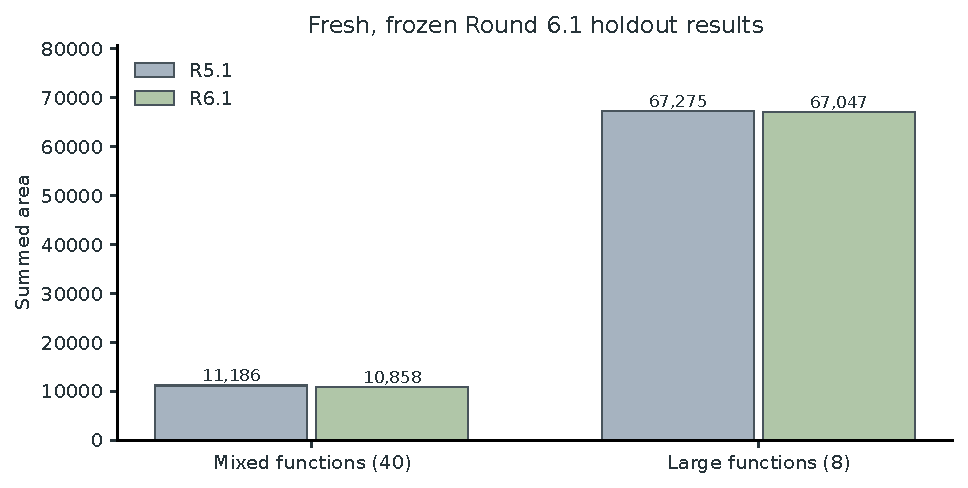
\includegraphics[width=.82\textwidth]{../shared/figures/holdout_area.pdf}
\caption{Fresh Round 6.1 holdout area by function family; source data and rendering script are included.}\end{figure}


\subsection{What the development budgets really measured}
We also recovered two intermediate budget sweeps. On the 40-function mixed \emph{development} set, the nominal cut budgets $25$, $35$ and $45$ ms all save the same $213$ local area units. The corresponding median \emph{postprocessor} wall times are $4.84$, $4.59$ and $4.91$ ms, a fluctuation too small to interpret as a monotone speed law. On a different, larger \emph{development} set of 16 functions, increasing the budget produces $358$, $408$ and $501$ area units saved, while median local wall time rises from $31.66$ to $40.89$ to $52.38$ ms.

\begin{figure}[H]\centering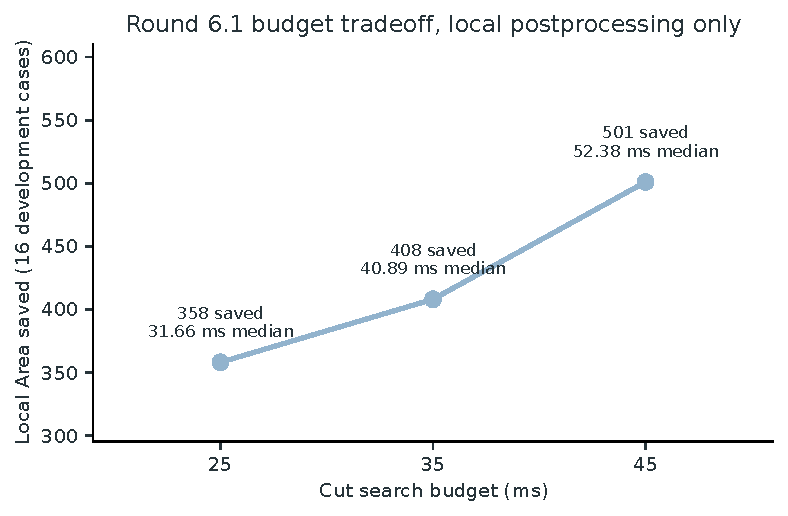
\includegraphics[width=.82\textwidth]{../shared/figures/round61_budget_tradeoff.pdf}
\caption{Larger-development-set Cut Budget experiment. ``Area saved'' measures the local postprocessor; these are not sums from the official Stage 1 evaluation.}\end{figure}

\textbf{Decision logic:} on easy local structures, more budget may buy nothing; on harder structures, it can buy more rewrites but at an increasing cost. That explains why the 25 ms limit was a defensible engineering compromise. It does not imply that 25 ms is optimal for every unknown truth table. These were \emph{development} sets already consulted during budget selection, so we cannot rebrand them as fresh blind holdouts.

\begin{tcolorbox}[colback=ResearchRose!16,colframe=ResearchRose,title=Decision after Round 6.1: No-Go for automatic promotion]
\textbf{Learning:} the hypothesis ``cut rewriting can reduce area'' is supported, while the stronger hypothesis ``the current bounded rewriting implementation is worth its runtime'' is rejected under our predeclared local criterion. The appropriate research response is to preserve the evidence and stop incremental threshold tuning, not to erase the unsuccessful branch.
\end{tcolorbox}

\section{How We Constructed Non-Official Test Cases}
\textbf{Motivation.} Repeatedly modifying a synthesizer after checking the same 25 Stage 1 inputs risks learning incidental features of those particular Boolean tables. More importantly, the public set alone cannot tell us whether an optimization helps affine parity-like functions, mux-heavy structures, sparse products, shared outputs, or dense random truth tables equally. We therefore constructed additional functions from \emph{generative descriptions} and only then expanded them into complete truth tables. This is not a new scoring system, and these cases are not professor-provided Stage 2 data.

\textbf{Construction.} A deterministic generator chooses a function family, a fixed pseudorandom seed, $n$ input variables, $m$ outputs, legal gate prices, and a delay target. For each assignment $x\in\{0,1\}^n$ it evaluates every output and serializes the resulting $m$-bit row. Thus the generator produces a legal complete instance, not a hand-selected Netlist. The mixed family includes affine functions (parity of selected inputs), sparse SOP, threshold functions, selector-based MUX, arithmetic bits, shared intermediate predicates, and dense deterministic truth bits. A separate large-function family composes local lookup tables, XORs, shared ensembles, and cascaded multiplexors. The scripts and case-hash manifests are preserved in \texttt{shared/test\_generation/}; the original truth tables are retained separately rather than redistributed in a public writing package.

\textbf{Evaluation protocol.} The Round 5.1 test record has an 80-case mixed set and a 16-case large structured set, plus 110 older regression cases and two stress cases. Round 6.1 was additionally evaluated on a newly seeded 40-case mixed set and an 8-case large set after its budget was selected. In contrast, the 25/35/45-ms cut-search budget sweep was conducted on development sets; it should not be mislabeled an untouched holdout. Each run checks functionality, legality, target delay, area, and synthesis time against the appropriate frozen comparator. A deterministic seed makes a suite repeatable but does not make it representative of an unknown deployment distribution.

\textbf{Research lesson.} A regression suite answers \emph{did this change break previously checked behavior?}; a frozen generated holdout asks \emph{does the promising trend persist on a different specified family?}; only the later official Stage 2 release will answer the separate question of generalization to the next course distribution. These distinctions stop an attractive Stage 1 result from being exaggerated into a universal claim.

\section{How did we guard against benchmark overfitting?}
A public benchmark is a finite development set. Repeatedly adjusting thresholds until its aggregate area decreases risks overfitting the properties of those 25 released functions. We therefore distinguish \emph{development evidence}, \emph{repeated regression tests}, and \emph{fresh generated holdouts} frozen after the candidate choices. Functions were generated from affine, sparse, threshold, multiplexing, arithmetic, dense and structured graph-related families across different sizes. Fresh holdout results were not used for further parameter tuning in the corresponding finalized experiments.

Nevertheless, there are limits. A synthetic generator creates its own distribution. A withheld seed is not equivalent to a future teacher-provided test distribution, and a collection already inspected during earlier iterations is no longer fully blind for later strategy decisions. We therefore claim only ``no observed functional regression on the tested families'' and, where supported, ``area improvement on the fresh holdouts.'' We do not claim statistical proof of optimality or of performance on unreleased Stage 2 cases.

Independent correctness verification adds a different kind of reassurance. The official evaluator performs the required truth-table check under its contract, while a separately written checker validates legality and independently simulates circuits. For selected smaller functions the independent checker enumerates all rows; for larger ones it uses deterministic samples. The latter is not a formal universal proof, and the separate mathematical correctness arguments are still important.

\section{A consolidated evidence narrative}
\subsection{The useful negative results}
Not every valid rewrite should be adopted. In the present study, a large truth-table-derived candidate pool could become impractically expensive; phase/algebra refinements produced diminishing public-case area gains; the smaller generated cases sometimes showed negligible runtime benefit from typed DAGs; and four-feasible cut rewriting reduced area but breached the local runtime-acceptance threshold. These observations are not defects to omit from a research record. Each separates a \emph{correct mathematical transform} from a \emph{justified engineering decision}. They also explain why further tuning of a public 25-case benchmark was stopped.

A particularly important counterfactual is the decision \emph{not} to promote R6.1. Had we selected the default solely by public-case area sum, we would have ignored its roughly 47.7\% local median-runtime penalty relative to R5.1. Had we dismissed it solely because of that penalty, we would have missed the independent evidence that cut rewriting can help other generated function families. Preserving the branch as an experimental result is more informative than either extreme.

\subsection{Why the version history needs more than one number}
\begin{figure}[H]\centering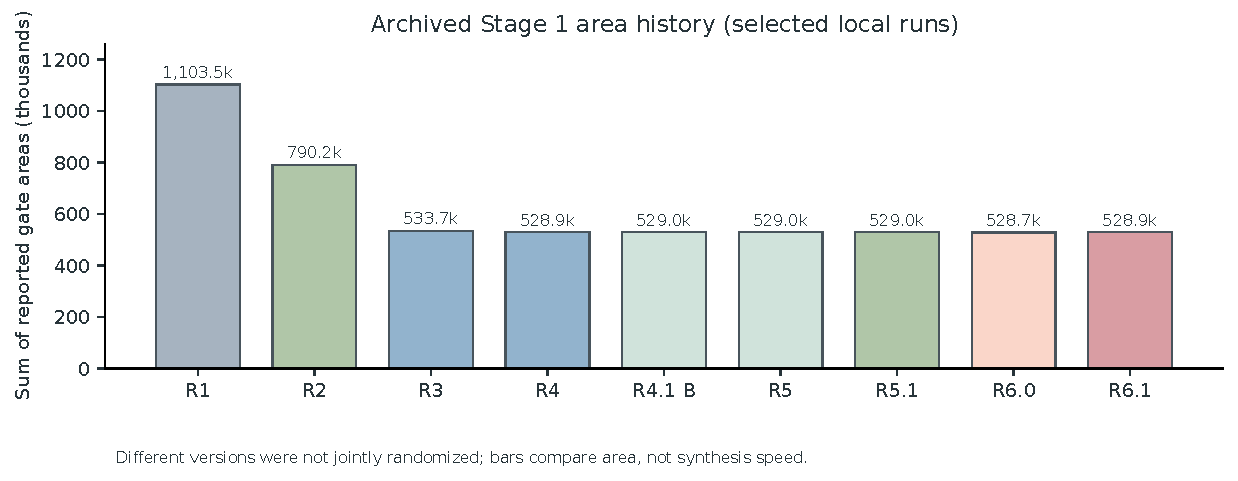
\includegraphics[width=.98\textwidth]{../shared/figures/area_evolution.pdf}
\caption{Selected archived local area totals. This is a non-paired development history; area totals are directly tabulated but runtime is not compared across archives.}\end{figure}

Read the sequence by the \emph{question solved}, not by the ordering of bar heights. R1 proves construction. R2 changes representations and meets the timing targets. R3 integrates the global deadline and reduces area substantially. R4 explores global phase and algebra, revealing expensive diminishing returns. R4.1 makes the Pareto tradeoff explicit. R5 and R5.1 refactor repeated computational work while preserving observed quality. R6.0 discovers an overlooked local area opportunity; R6.1 demonstrates the current technique's unfavorable cost under a fixed decision rule. These are complementary contributions, not a monotone sequence in all metrics.

\begin{table}[H]\centering\small\caption{Local Stage 1 area milestones; a single designated run per round}\begin{tabular}{@{}lrr@{}}\toprule
Round & Target met & Summed area \\ \midrule
1 &12/25&1,103,455\\
2 &25/25&790,243\\
3 &25/25&533,705\\
4 &25/25&528,910\\
4.1 Balanced &25/25&529,014\\
5 &25/25&529,014\\
\textbf{5.1 (default)}&\textbf{25/25}&\textbf{529,014}\\
6.0 (prototype)&25/25&528,738\\
6.1 (research)&25/25&528,854\\ \bottomrule\end{tabular}\end{table}

\subsection{What was not proved}
The work does not establish a globally minimum area or delay circuit for each input function. It does not show that lower delay after reaching target has zero score value; the numerical score formula was not published. A local gate-count reduction is not automatically a global area reduction in a shared DAG. BDD memory can be exponential. Synthesis time varies under CPU contention and wall-clock search cutoffs, so two valid runs can choose different candidates. These limitations should remain visible in any professional GitHub presentation.

\section{How to reconstruct the evidence and figures}
This writing archive includes all \emph{intermediate datasets used by its charts}, not only final images. Run \texttt{python shared/scripts/make\_figures.py} from the writing-package root (or call the script by absolute path); it reads the accompanying CSVs and the user-provided palette JSON. If the original local-results ZIP files are available, \texttt{python shared/scripts/extract\_evidence.py --source-dir /path/to/zips} rebuilds the normalized data from the official CSV members; \texttt{verify\_provenance.py} additionally checks exact archive digests and reconstructed output bytes. The SHA-256 archive provenance is retained in \texttt{source\_manifest.csv}. The student-verified research freeze identifies \texttt{synth\_round51.cpp}; its complete SHA-256 is in the bundled freeze manifest under \texttt{shared/data/raw\_evidence/}; this is not an assertion of a final Canvas submission.

A reproducible public repository should preserve each round's source snapshot, compiler flags, evaluator commands, input manifest/hash, official CSV, independent verification result, candidate outputs, and document with the research decision. Large raw netlists can be archived separately, while the paper still includes enough information for a reader to reproduce its figures. The exact local output paths follow the project's convention \texttt{local\_runs/YYYYMMDD\_HHMMSS\_Round*/report\_ready/}.


\subsection{A concrete replication exercise: from a saved official run to a plot}
A plot is not primary evidence. For example, the historical area timeline was derived from nine selected official CSVs stored in \emph{nine different local-run ZIPs}. Each row in the original CSV is an evaluator observation for one case, not an independently proved universal bound. To reconstruct the timeline properly, use the following sequence:
\begin{enumerate}[leftmargin=2em]
\item Identify the exact archive and CSV member in \texttt{shared/data/source\_manifest.csv}. Check the SHA-256 of the complete original ZIP; an archive with the same filename but different bytes is not automatically the same experiment.
\item Extract the 25 case rows and require unique case IDs \texttt{case\_001} through \texttt{case\_025}, with explicitly parsed \texttt{status}, \texttt{target\_met}, \texttt{area}, \texttt{delay}, and \texttt{runtime\_ms}. A functionally valid PASS can have \texttt{target\_met=no}.
\item Sum the 25 \texttt{area} values for the selected run. Compare the result to \texttt{round\_history.csv}, then regenerate \texttt{area\_evolution.pdf} using the packaged plotting script. This reproduces the \emph{displayed result}, not the original synthesis computation.
\item To reproduce synthesis itself, obtain the separate frozen C++ source, official input truth tables and Linux x86 evaluator, rebuild with the recorded flags, and run a fresh evaluation. Retain the new logs and use the independent checker on the resulting netlists. Because later candidates can be gated by wall-clock time, a new valid run need not produce the identical network bytes.
\end{enumerate}
The manuscript ZIP supplies the intermediate CSVs and plots; it \emph{does not} supply the instructor-restricted truth tables or the complete original local-run ZIPs. The additional \texttt{verify\_provenance.py} can audit only the first and third layers without original archives; passing that restricted audit is not evidence that the synthesis program itself was rerun.

\subsection{How we checked that the evidence was not silently rewritten}
For this review we ran the historical extraction program into an independent temporary directory. Fourteen normalized CSVs (nine selected official case tables, one run-history table, one manifest, one paired-benchmark table, one per-case comparison, and one holdout comparison) were byte-identical to the writing package. We also checked the standalone user-verified Round 5.1 source digest against the recorded manifest and the raw Round 3, Round 4 and Round 6.1 ablation input hashes. This verifies the lineage of those \emph{particular files}; it does not prove that a human-entered cutoff was chosen before observing every development result, nor does it establish statistical representativeness of synthetic holdouts.

For public GitHub presentation, we should publish the generic scripts, mathematical explanations, citation records, curated aggregate results (subject to course permission), and exact source provenance. We should \emph{not} assume permission to redistribute course-private full truth tables or the evaluator. These materials remain in private experiment archives, while the paper distinguishes available code from unavailable official inputs.


\section{Reflection and next steps}
\textbf{Research lesson.} A mathematical identity can certify equivalence; a cost model determines whether the identity is economically useful; a benchmark reports how a particular implementation behaved; and an adoption rule explains why that behavior warranted changing the default. Treating these as separate levels of reasoning is the central habit this project developed. The largest early improvements came from changing the search representation and acknowledging global timing; the later rounds taught us when \emph{not} to trade a large amount of computation for a tiny area gain.

The same small example clarifies what changes at each layer: a cofactor is a function, a BDD edge is a structural reference, a gate is a charged operation, and a path is a timed dependency. Reusing a reference, eliminating a live gate, and shortening a critical path are not interchangeable. This progression---Boolean function, shared decision graph, priced gate DAG, constrained timing graph, and resource-consuming search program---is the conceptual thread connecting the rounds.

An area-optimization algorithm can be mathematically sound and still be the wrong engineering choice when its marginal improvement is dwarfed by synthesis time. Preserving that negative result demonstrates an appropriate stopping criterion, especially under a rubric that rewards deep understanding and justified conceptual application. We therefore freeze Round 5.1 as the principal Stage 1 engineering baseline and preserve Rounds 6.0/6.1 as exploration branches, subject to the students' final submission choice.

For the later Stage 2 release, we should not reuse the published Stage 1 cases as though they were new holdouts. The actual submitted Stage 1 source should first be frozen, then both the old and any improved algorithm can be evaluated on the new release and on the original cases under matched conditions. This future work is outside the current Stage 1 record.


\section{Collaboration, AI-Assisted Development, and Responsibility}
\subsection{How the two students collaborated}
The two named student authors, Jincan LI and Zeyun DU, initially investigated approaches independently. They then compared ideas and integrated selected methods into a common research direction. This process was not divided into a fixed checklist of per-person ownership for BDDs, area recovery, or experimentation. We therefore describe the collaboration as independent exploration followed by mutual review and integration, without claiming that a specific individual authored each C++ module or mathematical derivation.

\subsection{What AI actually did}
Generative AI tools, principally ChatGPT, played a substantial role throughout the work. In particular, AI produced or substantially revised significant C++ implementation code, developed scripts for case execution, benchmarking, data gathering, verification and result packaging, and assisted in mathematical explanation, design suggestions, interpretation of measurements, and the preparation and iterative editing of these documents. This was not merely grammar correction, boilerplate generation, or occasional syntax help. The research record deliberately retains the generated tools and the results they produced rather than retroactively portraying the workflow as manual-only development.

\subsection{What the human review and local evidence contribute}
Human participation focused on asking which technical problem was worth solving next, questioning proposed optimizations and their marginal benefits, assessing the area--runtime trade-off, demanding checks against overfitting, and deciding when to keep or stop an approach. A student author independently executed the provided Linux evaluator and the local reproduction workflow in WSL, inspected the resulting summaries, and verified the chosen Round 5.1 source digest. These actions establish a concrete review and reproduction path; they do not support a claim that every line of code was written unaided or individually inspected in full.

Several risks follow directly from extensive AI assistance: an apparently plausible transformation may violate a graph invariant, a generated script may compare unmatched experimental runs, and a polished explanation may overstate what data establish. Our response was to retain source snapshots, evaluator outputs and independent checks, distinguish proofs from empirical findings, and revise claims whenever the evidence was narrower than an initial interpretation. This process improves traceability but cannot guarantee optimality or correctness on every unseen case. The authors remain responsible for the factual claims, appropriate citations, and final research decisions in any submitted or published version.

\bibliographystyle{IEEEtran}
\bibliography{../shared/bibliography/references}
\end{document}
